\section{Data \& API Design}
\label{sec:data_api}

\subsection{Hybrid Offline-First Data Architecture \& Data Dictionary}
\label{subsec:data_dictionary}

The data persistence layer of \textbf{Naomi} follows a \textbf{Hybrid Offline-First} paradigm spanning three synchronised storage domains: (1) \textbf{Supabase Cloud PostgreSQL} as the single source of truth for user identity, cloud bookmarks, reading history, and genre-audio mappings; (2) \textbf{MangaDex REST API v5 \& MangaDex@Home CDN} as the global comic metadata and page-image provider; and (3) \textbf{On-Device SQLite (Drift) + Sandboxed File Storage} for instant local reads and full offline operation. Table~\ref{tab:data_dictionary} summarises the 10 normalised relational tables.

\begin{table}[H]
\centering
\caption{System Data Dictionary across the 10 normalised tables of the Naomi database schema.}
\label{tab:data_dictionary}
\footnotesize
\renewcommand{\arraystretch}{1.22}
\begin{tabularx}{\textwidth}{C{0.7cm} L{3.1cm} L{2.8cm} Y C{2.2cm}}
\toprule
\rowcolor{tablehead}
\textbf{\#} & \textbf{Table Name} & \textbf{Storage Location} & \textbf{Primary Purpose \& Entity Role} & \textbf{FR Mapping} \\
\midrule
1 & \texttt{users} & Supabase Cloud & User profile linked 1:1 to \texttt{auth.users(id)}, display name, avatar, and JSONB UI preferences. & \texttt{FR-00, FR-14} \\
\rowcolor{tablerow}
2 & \texttt{comics} & Cloud \& Local Cache & Comic series metadata (title, alt\_title, author, artist, status, cover\_url, default ambient track). & \texttt{FR-01, FR-08, FR-10} \\
3 & \texttt{genres} & Cloud \& Local Cache & Canonical genre catalogue (\texttt{action, fantasy, romance, slice\_of\_life}, etc.). & \texttt{FR-01, FR-05} \\
\rowcolor{tablerow}
4 & \texttt{comic\_genres} & Cloud \& Local Cache & Associative $M\text{:}N$ join table linking \texttt{comics} and \texttt{genres} via composite PK. & \texttt{FR-01, FR-05} \\
5 & \texttt{chapters} & Cloud \& Local Cache & Individual chapter metadata (chapter\_number, volume, title, page\_count, optional audio override). & \texttt{FR-02, FR-04, FR-10} \\
\rowcolor{tablerow}
6 & \texttt{pages} & Cloud \& Local Cache & \textbf{Weak Entity} representing ordered pages within a chapter, identified by \texttt{(chapter\_id, page\_number)}. & \texttt{FR-02, FR-03} \\
7 & \texttt{ambient\_tracks} & Supabase DB/Storage & Instrumental background tracks categorised by genre with streaming MP3 URLs and loop metadata. & \texttt{FR-05, FR-09} \\
\rowcolor{tablerow}
8 & \texttt{reading\_history} & Cloud \& Local SQLite & Exact page-level progress (\texttt{last\_page\_read}, \texttt{read\_percentage}, \texttt{is\_synced}); strictly 3NF. & \texttt{FR-04, FR-08} \\
9 & \texttt{bookmarks} & Cloud \& Local SQLite & User's personal bookmarked series (\texttt{is\_favorite}, \texttt{reading\_status}) synced across devices. & \texttt{FR-07, FR-10} \\
\rowcolor{tablerow}
10 & \texttt{offline\_downloads} & Local SQLite Only & Tracks local chapter download status, byte size, and relative directory path in sandboxed storage; strictly 3NF. & \texttt{FR-06, FR-07, FR-13} \\
\bottomrule
\end{tabularx}
\end{table}

\subsection{Conceptual \& Physical Entity-Relationship Diagrams}
\label{subsec:erd_diagrams}

Following standard database design methodology (\textit{Elmasri \& Navathe, Fundamentals of Database Systems, 7th Ed., Chapters 2--3}), Figure~\ref{fig:erd_chen} presents the \textbf{Conceptual Entity-Relationship Diagram in Chen Notation} (highlighting strong vs.\ weak entities, identifying relationships, total participation double lines, and partial key dashed underlines), while Figure~\ref{fig:erd_crowsfoot} presents the mapped \textbf{Physical Relational Schema in Crow's Foot Notation}.

\begin{figure}[H]
    \centering
    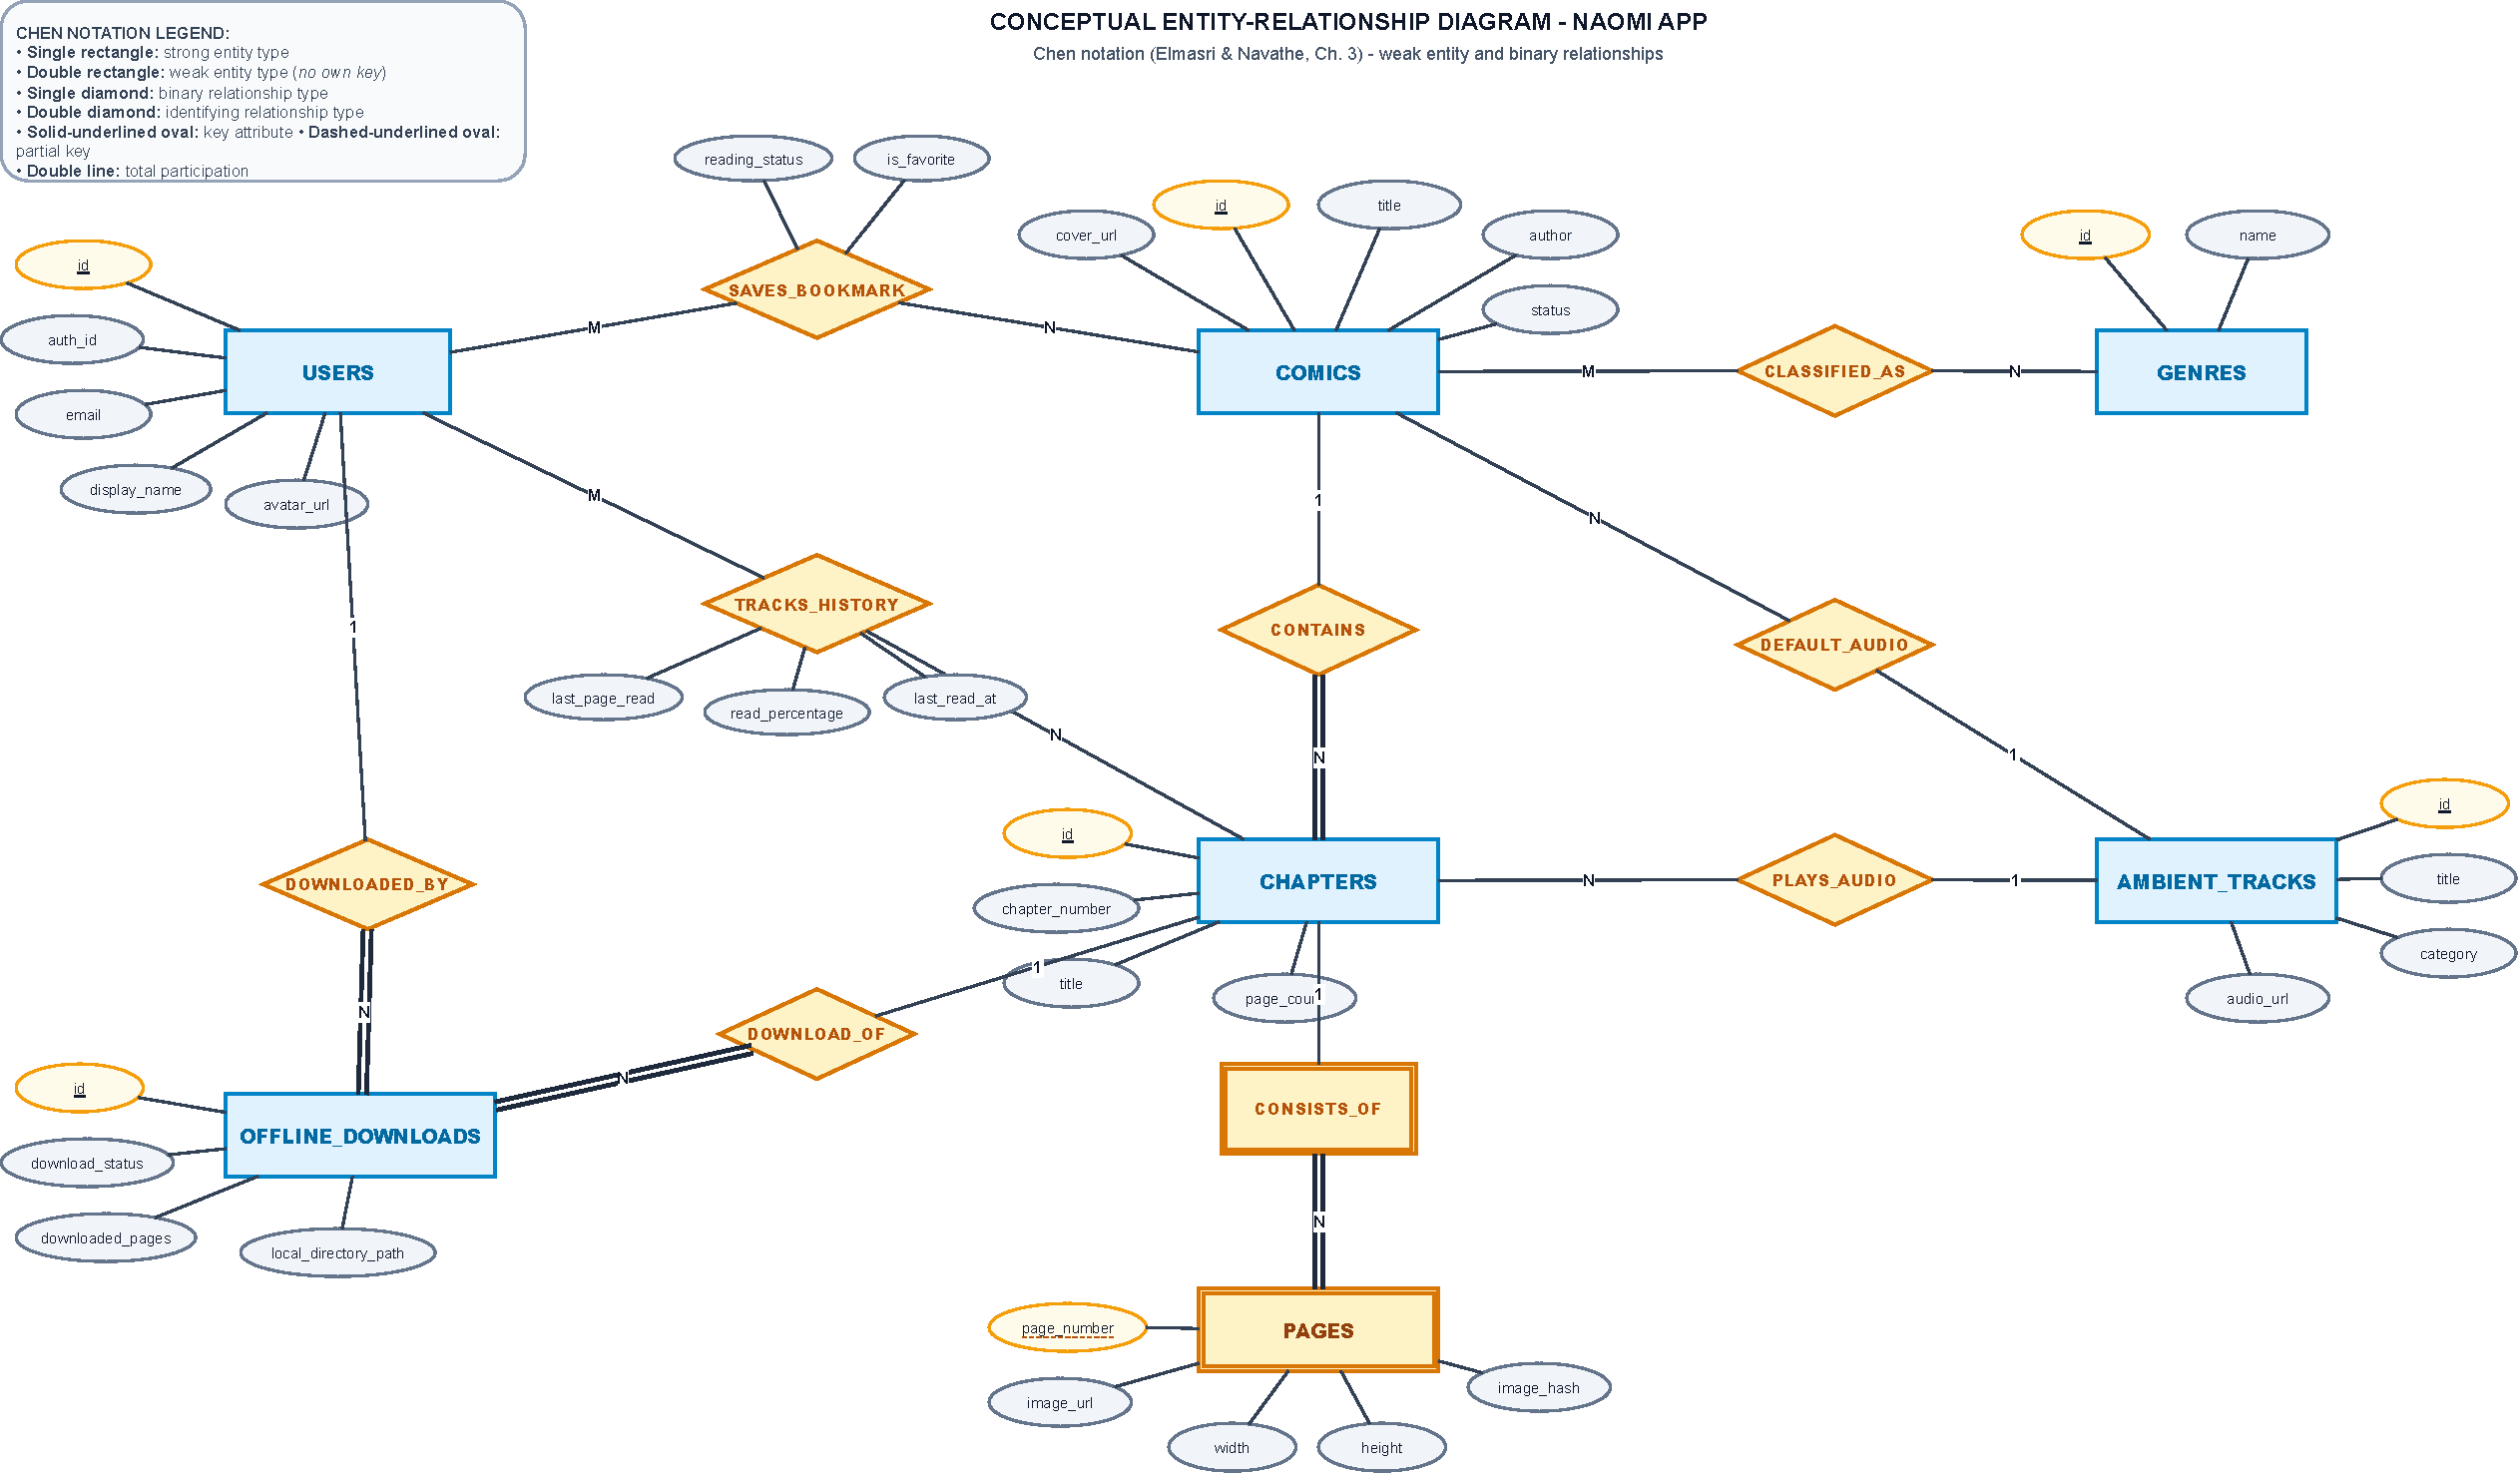
\includegraphics[width=0.99\textwidth]{figures/diagrams/erd_conceptual_chen.pdf}
    \caption{Conceptual Entity-Relationship Diagram (Chen Notation) illustrating strong entities, the weak entity \texttt{PAGES} with partial key \texttt{page\_number}, and binary relationships.}
    \label{fig:erd_chen}
\end{figure}

\begin{figure}[H]
    \centering
    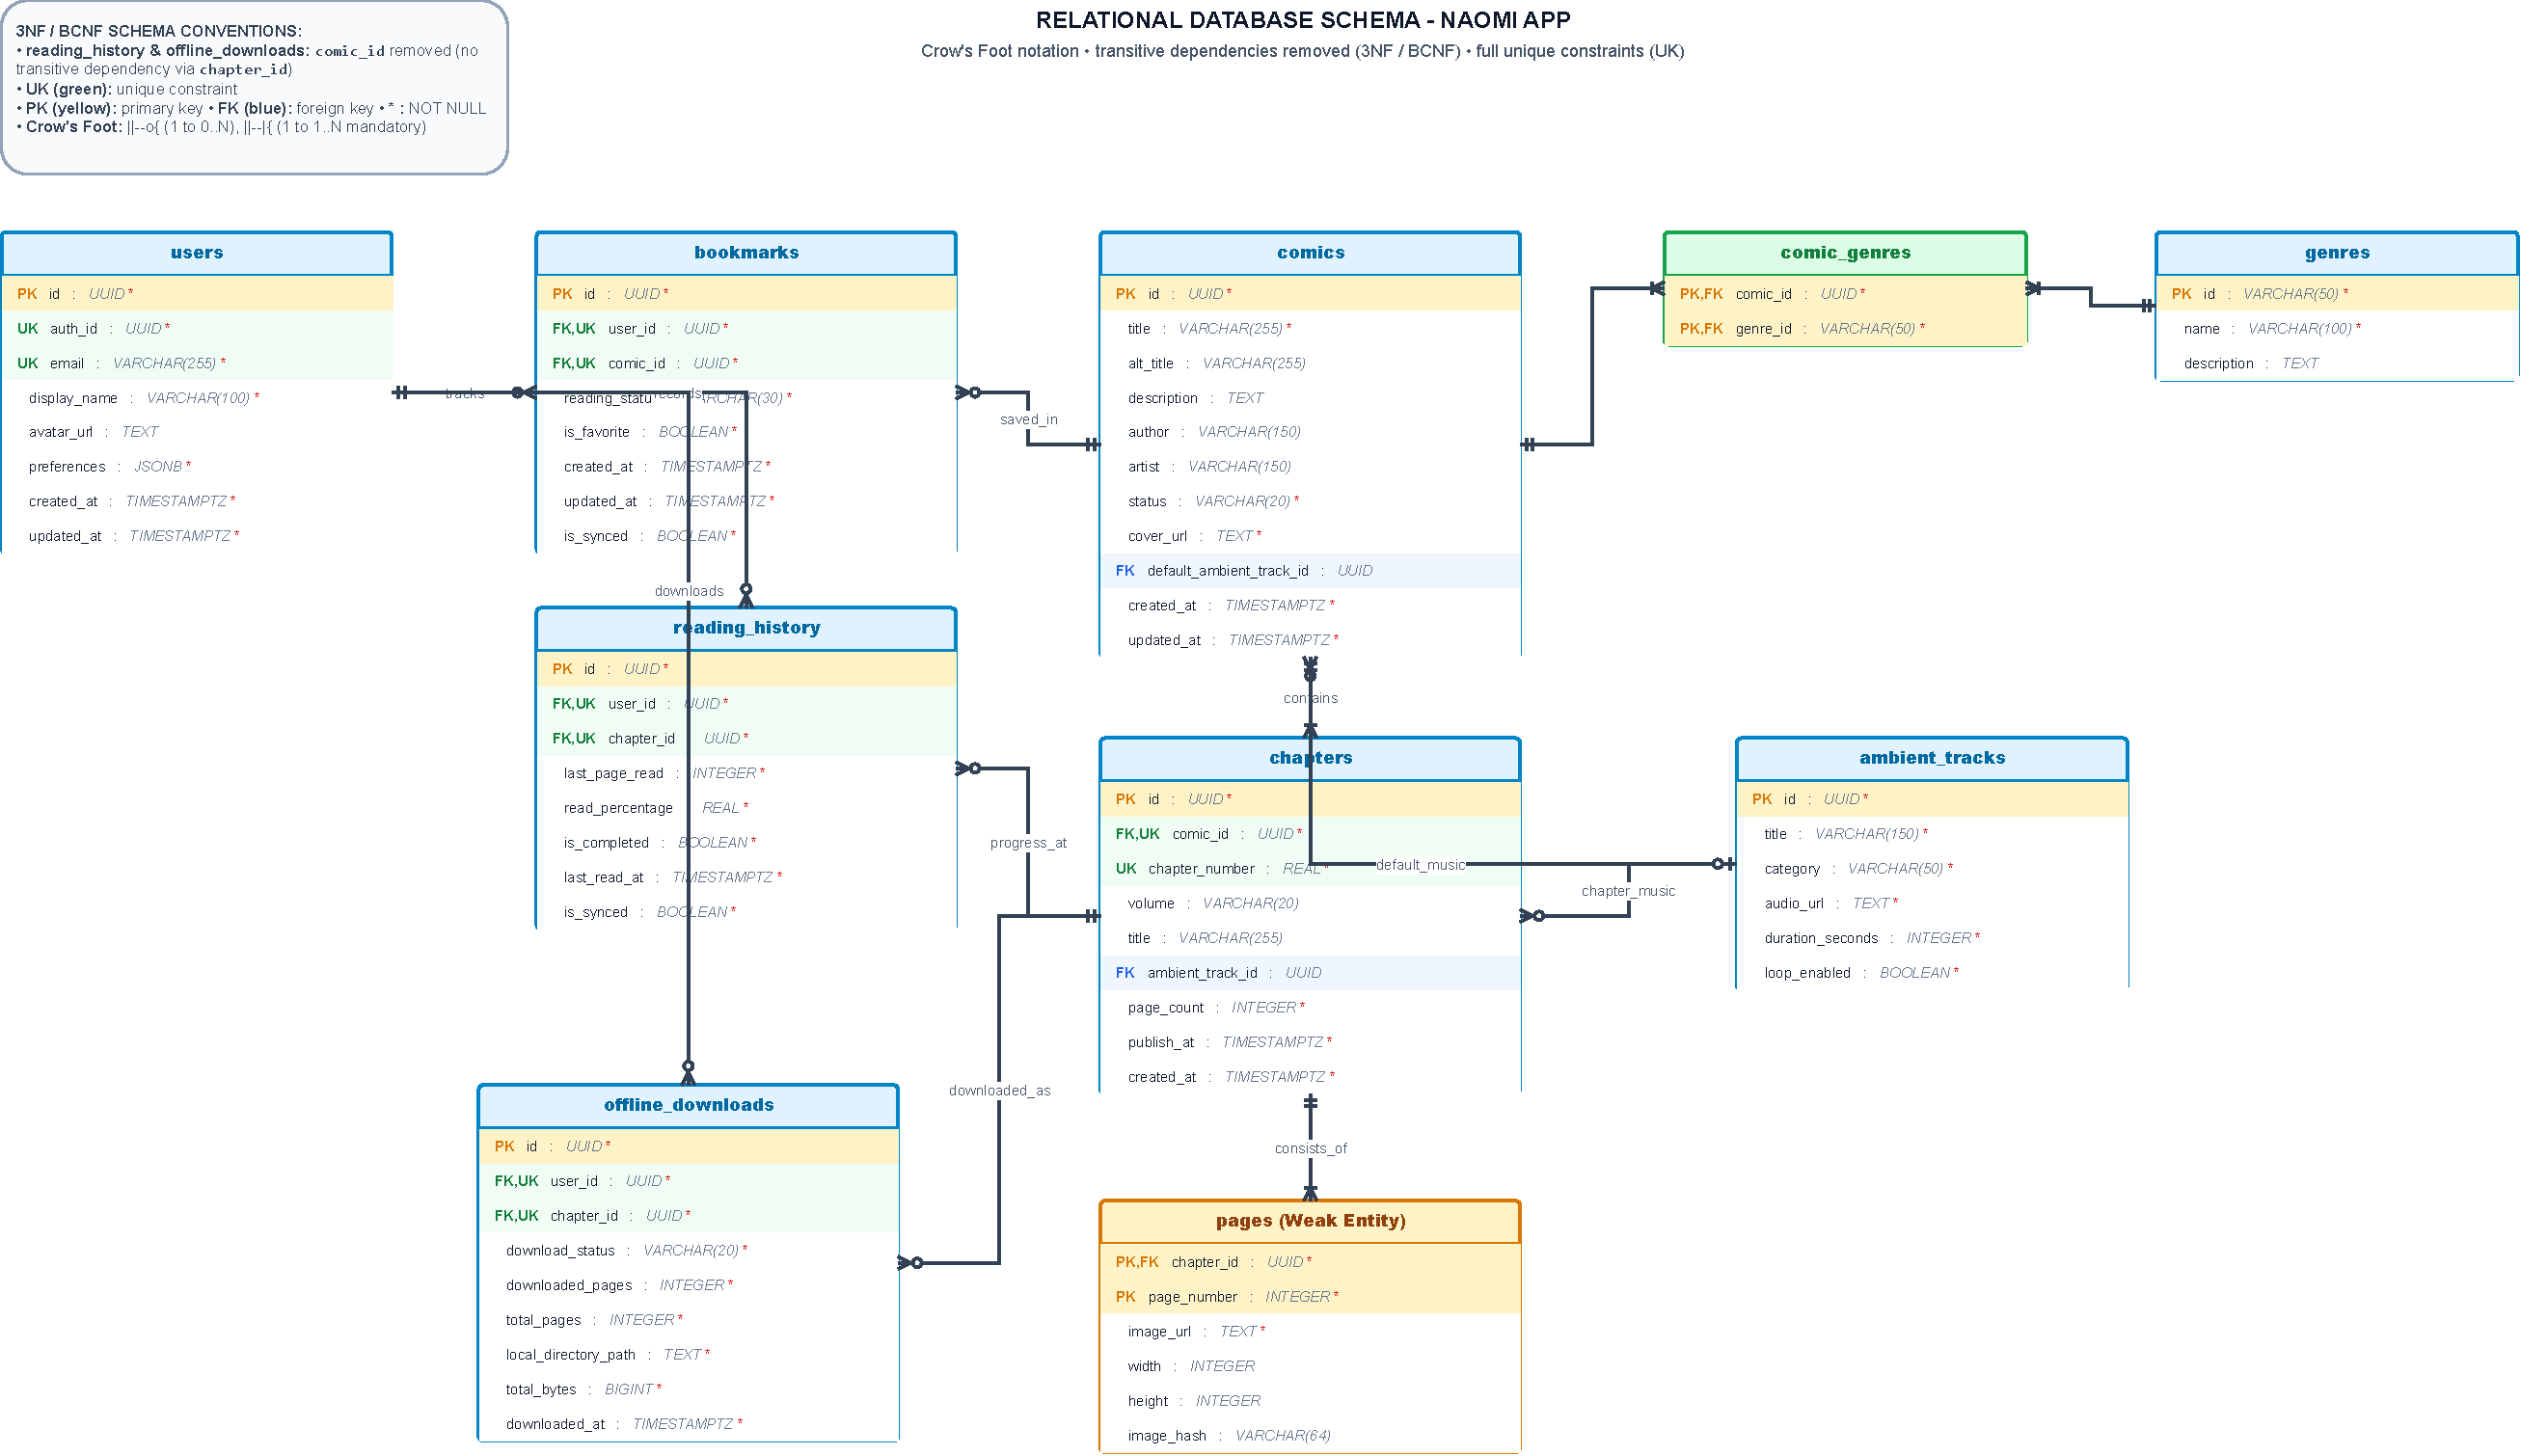
\includegraphics[width=0.99\textwidth]{figures/diagrams/erd_relational_crowsfoot.pdf}
    \caption{Physical Relational Database Schema (Crow's Foot Notation) enforcing 3NF/BCNF, Primary Keys (PK), Foreign Keys (FK), and Unique Constraints (UK).}
    \label{fig:erd_crowsfoot}
\end{figure}

\subsection{Detailed Relational Schema, 3NF/BCNF Normalisation Proof \& RLS Security}
\label{subsec:schema_norm_rls}

\subsubsection{Relational Schema Specifications (10 Tables)}
\begin{itemize}
    \item \textbf{\texttt{users}:} \texttt{id UUID PK}, \texttt{auth\_id UUID UNIQUE NOT NULL}, \texttt{email VARCHAR(255) UNIQUE NOT NULL}, \texttt{display\_name VARCHAR(100) NOT NULL}, \texttt{avatar\_url TEXT}, \texttt{preferences JSONB DEFAULT} \allowbreak \texttt{'\{"scroll\_direction":} \allowbreak \texttt{"vertical",} \allowbreak \texttt{"ambient\_auto\_play":} \allowbreak \texttt{true,} \allowbreak \texttt{"ambient\_volume":0.3\}'}, \texttt{created\_at TIMESTAMPTZ}, \texttt{updated\_at TIMESTAMPTZ}.
    \item \textbf{\texttt{comics}:} \texttt{id UUID PK}, \texttt{title VARCHAR(255) NOT NULL}, \texttt{alt\_title VARCHAR(255)}, \texttt{description TEXT}, \texttt{author VARCHAR(150)}, \texttt{artist VARCHAR(150)}, \texttt{status VARCHAR(20) CHECK (status IN ('ongoing','completed','hiatus','cancelled'))}, \texttt{cover\_url TEXT NOT NULL}, \texttt{default\_ambient\_track\_id UUID} \allowbreak \texttt{FK $\to$ ambient\_tracks(id) ON DELETE SET NULL}, \texttt{created\_at}, \texttt{updated\_at}.
    \item \textbf{\texttt{genres} \& \texttt{comic\_genres}:} \texttt{genres(id VARCHAR(50) PK, name VARCHAR(100) NOT NULL, description TEXT)}; \texttt{comic\_genres(comic\_id UUID FK, genre\_id VARCHAR(50) FK,} \allowbreak \texttt{PRIMARY KEY (comic\_id, genre\_id))}.
    \item \textbf{\texttt{chapters}:} \texttt{id UUID PK}, \texttt{comic\_id UUID NOT NULL FK $\to$ comics(id) ON DELETE CASCADE}, \texttt{chapter\_number REAL NOT NULL}, \texttt{volume VARCHAR(20)}, \texttt{title VARCHAR(255)}, \texttt{ambient\_track\_id UUID FK $\to$ ambient\_tracks(id) ON DELETE SET NULL}, \texttt{page\_count INT NOT NULL}, \texttt{publish\_at TIMESTAMPTZ}, \texttt{created\_at TIMESTAMPTZ}, with \texttt{UNIQUE(comic\_id, chapter\_number)}.
    \item \textbf{\texttt{pages} (Weak Entity Mapping):} \texttt{chapter\_id UUID NOT NULL FK $\to$ chapters(id) ON DELETE CASCADE}, \texttt{page\_number INT NOT NULL}, \texttt{image\_url TEXT NOT NULL}, \texttt{width INT}, \texttt{height INT}, \texttt{image\_hash VARCHAR(64)}, with composite \texttt{PRIMARY KEY} \allowbreak \texttt{(chapter\_id, page\_number)}.
    \item \textbf{\texttt{ambient\_tracks}:} \texttt{id UUID PK}, \texttt{title VARCHAR(150) NOT NULL}, \texttt{category VARCHAR(50) NOT NULL}, \texttt{audio\_url TEXT NOT NULL}, \texttt{duration\_seconds INT NOT NULL}, \texttt{loop\_enabled BOOLEAN DEFAULT TRUE}.
    \item \textbf{\texttt{reading\_history} (3NF/BCNF):} \texttt{id UUID PK}, \texttt{user\_id UUID NOT NULL FK $\to$ users(id) ON DELETE CASCADE}, \texttt{chapter\_id UUID NOT NULL FK $\to$ chapters(id) ON DELETE CASCADE}, \texttt{last\_page\_read INT NOT NULL DEFAULT 1}, \texttt{read\_percentage REAL NOT NULL DEFAULT 0.0}, \texttt{is\_completed BOOLEAN DEFAULT FALSE}, \texttt{last\_read\_at TIMESTAMPTZ}, \texttt{is\_synced BOOLEAN DEFAULT TRUE}, with \texttt{UNIQUE(user\_id, chapter\_id)}.
    \item \textbf{\texttt{bookmarks}:} \texttt{id UUID PK}, \texttt{user\_id UUID NOT NULL FK $\to$ users(id) ON DELETE CASCADE}, \texttt{comic\_id UUID NOT NULL FK $\to$ comics(id) ON DELETE CASCADE}, \texttt{reading\_status VARCHAR(30) DEFAULT 'reading'}, \texttt{is\_favorite BOOLEAN DEFAULT FALSE}, \texttt{created\_at}, \texttt{updated\_at}, \texttt{is\_synced BOOLEAN}, with \texttt{UNIQUE(user\_id, comic\_id)}.
    \item \textbf{\texttt{offline\_downloads} (3NF/BCNF):} \texttt{id UUID PK}, \texttt{user\_id UUID NOT NULL FK $\to$ users(id) ON DELETE CASCADE}, \texttt{chapter\_id UUID NOT NULL FK $\to$ chapters(id) ON DELETE CASCADE}, \texttt{download\_status VARCHAR(20) CHECK (download\_status IN} \allowbreak \texttt{('pending','downloading',} \allowbreak \texttt{'completed','failed'))}, \texttt{downloaded\_pages INT}, \texttt{total\_pages INT NOT NULL}, \texttt{local\_directory\_path TEXT NOT NULL}, \texttt{total\_bytes BIGINT}, \texttt{downloaded\_at TIMESTAMPTZ}, with \texttt{UNIQUE(user\_id, chapter\_id)}.
\end{itemize}

\subsubsection{Formal 3NF \& Boyce-Codd Normal Form (BCNF) Proof}
\begin{enumerate}
    \item \textbf{First Normal Form (1NF):} Every attribute across all 10 relations holds atomic values. Multi-valued genre tags are decomposed into the associative relation \texttt{comic\_genres(comic\_id, genre\_id)}.
    \item \textbf{Second Normal Form (2NF):} All single-attribute UUID primary keys are trivially free of partial dependencies. For composite-key tables---\texttt{comic\_genres(comic\_id, genre\_id)} (no non-key attributes) and the weak entity \texttt{pages(chapter\_id, page\_number)}---every non-key attribute (\texttt{image\_url, width, height, image\_hash}) depends irreducibly on both \texttt{chapter\_id} and \texttt{page\_number}.
    \item \textbf{Third Normal Form (3NF) \& BCNF:} Because every chapter belongs to exactly one comic ($\text{chapter\_id} \to \text{comic\_id}$), storing \texttt{comic\_id} inside \texttt{reading\_history} or \texttt{offline\_downloads} would introduce the transitive functional dependency $\text{id} \to \text{chapter\_id} \to \text{comic\_id}$. Our schema \textbf{explicitly eliminates \texttt{comic\_id} from both \texttt{reading\_history} and \texttt{offline\_downloads}}, resolving parent comic metadata via an indexed join on \texttt{chapters(comic\_id)}. Similarly, audio metadata is factored out into \texttt{ambient\_tracks}. Consequently, for every non-trivial functional dependency $X \to Y$ across all 10 tables, $X$ is a superkey, proving strict compliance with \textbf{BCNF} (\textit{Elmasri \& Navathe, Ch.\ 5}).
\end{enumerate}

\subsubsection{Database Security \& Row-Level Security (RLS) Policies}
To enforce tenant isolation at the database engine level (\texttt{NFR-10}, \texttt{NFR-11}), Supabase PostgreSQL Row-Level Security is enabled across all user-data tables:

\begin{lstlisting}[language=SQL,caption={Supabase PostgreSQL Row-Level Security (RLS) Policies for User Isolation.}]
ALTER TABLE users ENABLE ROW LEVEL SECURITY;
ALTER TABLE reading_history ENABLE ROW LEVEL SECURITY;
ALTER TABLE bookmarks ENABLE ROW LEVEL SECURITY;

-- 1. USERS: Users can only SELECT, INSERT, or UPDATE their own profile row
CREATE POLICY "Users view own profile" ON users FOR SELECT USING (auth.uid() = auth_id);
CREATE POLICY "Users insert own profile" ON users FOR INSERT WITH CHECK (auth.uid() = auth_id);
CREATE POLICY "Users update own profile" ON users FOR UPDATE USING (auth.uid() = auth_id);

-- 2. READING_HISTORY & BOOKMARKS: Strict per-user isolation via auth.uid()
CREATE POLICY "Users manage own reading history" ON reading_history FOR ALL
  USING (auth.uid() = (SELECT auth_id FROM users WHERE users.id = reading_history.user_id));

CREATE POLICY "Users manage own bookmarks" ON bookmarks FOR ALL
  USING (auth.uid() = (SELECT auth_id FROM users WHERE users.id = bookmarks.user_id));

-- 3. PUBLIC CATALOG TABLES: Read-only access for authenticated and anonymous clients
ALTER TABLE comics ENABLE ROW LEVEL SECURITY;
CREATE POLICY "Public read-only comics" ON comics FOR SELECT USING (true);
\end{lstlisting}

\subsection{On-Device 4-Tier Storage \& Bidirectional Sync Strategy}
\label{subsec:local_storage_strategy}

Table~\ref{tab:storage_tiers} defines the \textbf{4-Tier Mobile Storage Strategy} deployed on the client device. Crucially, \textbf{binary image and audio files are never stored as SQLite BLOBs} (which would bloat database pages and cause OOM crashes, violating \texttt{NFR-03} and \texttt{NFR-06}); all media assets reside on the sandboxed file system while SQLite stores only indexed relative file paths.

\begin{table}[H]
\centering
\caption{4-Tier On-Device Mobile Persistence and Eviction Strategy.}
\label{tab:storage_tiers}
\footnotesize
\renewcommand{\arraystretch}{1.22}
\begin{tabularx}{\textwidth}{L{2.5cm} L{3.3cm} L{3.5cm} Y}
\toprule
\rowcolor{tablehead}
\textbf{Storage Tier} & \textbf{Engine / API} & \textbf{Persisted Data} & \textbf{Security \& Eviction Policy} \\
\midrule
\textbf{Tier 1: Secure Credentials} & \texttt{flutter\_\allowbreak secure\_\allowbreak storage} & Supabase JWT \texttt{access\_\allowbreak token}, \texttt{refresh\_\allowbreak token} & \textbf{AES-256 hardware encryption} (Keystore / Keychain); wiped immediately on \textit{Sign Out} (\texttt{S08}). \\
\rowcolor{tablerow}
\textbf{Tier 2: Relational Metadata} & \texttt{Drift} (SQLite ORM) & Cached metadata, \texttt{reading\_\allowbreak history}, \texttt{bookmarks}, \texttt{offline\_\allowbreak downloads}, sync queue & App-private sandboxed DB; retained across restarts; indexed for $\le 50\text{ ms}$ queries (\texttt{NFR-09}). \\
\textbf{Tier 3: Offline Downloads} & \texttt{Application\allowbreak DocumentsDir} & Downloaded chapter pages (\texttt{.webp}) for offline reading & Protected from automatic cache eviction; user-managed via \texttt{S07} (\textit{Offline Reading}). \\
\rowcolor{tablerow}
\textbf{Tier 4: Dynamic Disk Cache} & \texttt{Temporary\allowbreak Directory} + \texttt{cached\_\allowbreak network\_\allowbreak image} & Transient online covers, preloaded chapter pages, audio buffers & \textbf{LRU Eviction (\texttt{NFR-07}):} hard cap at $500\text{ MB}$ (auto-pruned to $350\text{ MB}$) or manual clear on \texttt{S08}. \\
\bottomrule
\end{tabularx}
\end{table}

\textbf{Bidirectional Offline-First Synchronisation Algorithm:} Whenever the user reads or bookmarks while offline, records are written to local SQLite with \texttt{is\_synced = FALSE} and \texttt{last\_read\_at = NOW()}. Upon network restoration (detected via \texttt{ConnectivityPlus}), a background sync worker batches all unsynced rows to Supabase via \texttt{POST /rest/v1/reading\_history} using a \textbf{Last-Write-Wins (LWW)} timestamp resolution rule before setting \texttt{is\_synced = TRUE}.

\subsection{RESTful API Contract Specification \& Error Code Dictionary}
\label{subsec:api_contract}

All remote communications use \texttt{HTTPS / TLS 1.3} with JSON payloads (\texttt{application/json; charset=utf-8}). Table~\ref{tab:api_overview} summarises the seven core API endpoints across \textbf{MangaDex REST API v5} (\texttt{https://api.mangadex.org}) and \textbf{Supabase Backend Services} (\texttt{https://[project-id].supabase.co}), followed by representative payload schemas and the standardized Error Code Dictionary (Table~\ref{tab:error_codes}).

\begin{table}[H]
\centering
\caption{Catalogue of the 7 RESTful API Endpoints across MangaDex v5 and Supabase Backend.}
\label{tab:api_overview}
\footnotesize
\renewcommand{\arraystretch}{1.22}
\begin{tabularx}{\textwidth}{C{1.2cm} L{4.6cm} L{2.8cm} Y C{1.8cm}}
\toprule
\rowcolor{tablehead}
\textbf{API ID} & \textbf{Method \& Endpoint Path} & \textbf{Provider} & \textbf{Request Parameters / Headers \& Purpose} & \textbf{FR / NFR} \\
\midrule
\textbf{API 01} & \texttt{GET /manga} & MangaDex v5 & Query: \texttt{title}, \texttt{includedTags[]}, \texttt{limit=20}, \texttt{offset}, \texttt{order[rating]=desc}. Searches \& filters comics. & \texttt{FR-01, FR-08, FR-11} \\
\rowcolor{tablerow}
\textbf{API 02} & \texttt{GET /manga/\{id\}/feed} & MangaDex v5 & Query: \texttt{translatedLanguage[]=en,vi}, \texttt{order[chapter]=asc}, \texttt{limit=100}. Fetches ordered chapter feed. & \texttt{FR-02, FR-10} \\
\textbf{API 03} & \texttt{GET /at-home/} \allowbreak \texttt{server/\{chapterId\}} & MangaDex@Home & Resolves CDN \texttt{baseUrl}, \texttt{hash}, high-res \texttt{data[]}, and compressed \texttt{dataSaver[]} page filenames. & \texttt{FR-02, FR-06, NFR-18} \\
\rowcolor{tablerow}
\textbf{API 04} & \texttt{POST /auth/v1/token}\newline \texttt{POST /auth/v1/signup} & Supabase Auth & Header: \texttt{apikey}. Body: \texttt{\{email, password\}} or \texttt{\{refresh\_token\}}. Issues JWT Bearer session. & \texttt{FR-00, NFR-05, NFR-10} \\
\textbf{API 05} & \texttt{POST /rest/v1/} \allowbreak \texttt{reading\_history} & Supabase REST & Header: \texttt{Bearer JWT}, \texttt{Prefer: resolution=merge-duplicates}. Upserts page-level reading progress. & \texttt{FR-04, NFR-09} \\
\rowcolor{tablerow}
\textbf{API 06} & \texttt{GET | POST | DELETE} \allowbreak \texttt{/rest/v1/bookmarks} & Supabase REST & Header: \texttt{Bearer JWT}. CRUD operations on user's cloud-synced \textit{Favorites} library. & \texttt{FR-07, FR-10} \\
\textbf{API 07} & \texttt{GET /rest/v1/} \allowbreak \texttt{ambient\_tracks} & Supabase REST & Query: \texttt{category=eq.\{genre\}}. Returns genre-matched instrumental MP3 streaming URLs. & \texttt{FR-05, FR-09} \\
\bottomrule
\end{tabularx}
\end{table}

\begin{lstlisting}[language=json,caption={Representative Request/Response Schemas for API 03 (MangaDex@Home CDN), API 04 (Supabase Auth), API 05 (Reading Progress Upsert), and API 07 (Genre Ambient Audio).}]
// 1. API 03 Response: GET https://api.mangadex.org/at-home/server/{chapterId} (HTTP 200 OK)
// Page URL construction: {baseUrl}/data/{hash}/{fileName} (or /data-saver/ on 4G cellular)
{
  "result": "ok",
  "baseUrl": "https://cmdxd98sb0x3yprd.mangadex.network",
  "chapter": {
    "hash": "a823f99c15e8bc42f2b3b0d23c10",
    "data": ["page_001.webp", "page_002.webp", "page_042.webp"],
    "dataSaver": ["page_001.jpg", "page_002.jpg", "page_042.jpg"]
  }
}

// 2. API 04 Response: POST https://[project].supabase.co/auth/v1/token?grant_type=password (HTTP 200 OK)
{
  "access_token": "eyJhbGciOiJIUzI1NiIsInR5cCI6IkpXVCJ9...",
  "token_type": "bearer",
  "expires_in": 3600,
  "refresh_token": "f47ac10b-58cc-4372-a567-0e02b2c3d479",
  "user": {
    "id": "e4eaaaf2-d142-11e1-b3e4-080027620cdd",
    "email": "reader.kiet@gmail.com",
    "user_metadata": { "display_name": "Kiet Nguyen" }
  }
}

// 3. API 05 Request & Response: POST /rest/v1/reading_history (HTTP 201 Created)
{
  "user_id": "e4eaaaf2-d142-11e1-b3e4-080027620cdd",
  "chapter_id": "chapter-uuid-024",
  "last_page_read": 18,
  "read_percentage": 42.8,
  "is_completed": false,
  "last_read_at": "2026-11-04T12:00:00Z"
}

// 4. API 07 Response: GET /rest/v1/ambient_tracks?category=eq.fantasy (HTTP 200 OK)
[
  {
    "id": "track-uuid-fantasy-01",
    "title": "Winds of Aureole (Instrumental)",
    "category": "fantasy",
    "audio_url": "https://[project].supabase.co/storage/v1/object/public/ambient-audio/winds_aureole.mp3",
    "duration_seconds": 192,
    "loop_enabled": true
  }
]
\end{lstlisting}

\begin{table}[H]
\centering
\caption{System Error Code Dictionary and Deterministic UI/UX Recovery Actions.}
\label{tab:error_codes}
\footnotesize
\renewcommand{\arraystretch}{1.22}
\begin{tabularx}{\textwidth}{C{1.8cm} L{4.2cm} L{3.6cm} Y}
\toprule
\rowcolor{tablehead}
\textbf{HTTP Status} & \textbf{Internal Error Code} & \textbf{Technical Meaning} & \textbf{Presentation Layer (BLoC / UI) Recovery Action} \\
\midrule
\textbf{200 / 201} & \texttt{SUCCESS} & Request succeeded & Emit \texttt{LoadedState}; render data and update local SQLite cache. \\
\rowcolor{tablerow}
\textbf{204} & \texttt{NO\_CONTENT} & Resource deleted cleanly & Remove bookmark/item from UI state immediately. \\
\textbf{400} & \texttt{ERR\_BAD\_REQUEST} & Malformed input or invalid credentials & Display inline field validation error on \texttt{S01} while preserving user input. \\
\rowcolor{tablerow}
\textbf{401} & \texttt{ERR\_UNAUTHORIZED} & Expired or missing JWT token & Trigger silent token refresh (\texttt{API 04}); if refresh fails, route to \texttt{S01 Sign In}. \\
\textbf{403} & \texttt{ERR\_FORBIDDEN} & Supabase RLS policy violation & Block unauthorized cross-user mutation and log security event. \\
\rowcolor{tablerow}
\textbf{404} & \texttt{ERR\_NOT\_FOUND} & Comic or chapter unavailable & Render clean Empty State with a back navigation button. \\
\textbf{429} & \texttt{ERR\_RATE\_LIMITED} & Exceeded MangaDex $5\text{ req/s}$ limit & \texttt{Dio} interceptor executes automatic exponential backoff respecting \texttt{Retry-After}. \\
\rowcolor{tablerow}
\textbf{500} & \texttt{ERR\_INTERNAL\_SERVER} & Upstream server fault & Display non-blocking SnackBar with a 1-tap \textit{Retry} action. \\
\textbf{0 (No Net)} & \texttt{ERR\_NETWORK\_DISCONNECTED} & Complete loss of Internet connectivity & \textbf{Automatic Offline Fallback (\texttt{NFR-08} $\le 300\text{ ms}$):} serve cached chapters from SQLite or display \texttt{S09} routing to \texttt{S07 Offline Library}. \\
\bottomrule
\end{tabularx}
\end{table}
